%% Bachelor Thesis Template of Xidian Uniersity
%%   for using XDBAthesis package with LaTeX
%%
%% Created by Xue-Jilong(xuejilong@gmail.com)
%%
%% template.tex v0.1, 2011/03/21


\documentclass[xetex,adobefonts,master]{XDBAthesis}
% 选项说明:
% dvipdfm  使用 dvipdfm(x) 生成最终的 PDF 文档 (缺省设置)
% dvips    使用 dvips 生成最终的 PS 文档
% pdftex   使用 pdfLaTeX 生成最终的 PDF 文档
% xetex    使用 XeLaTeX 生成 PD F文档
% adobefonts 使用 Adobe 中文字体
% winfonts 使用 Windows 中文字体
% master   用于生成硕士学位论文

% 图形文件的搜索路径
\graphicspath{{chapter-utf8/}{figures/}}

\begin{document}
%%----------------- 封面部分 ----------------- %%
    \schoolnumber{07071050}
    \title{复杂网络的数学模型研究与应用}{}   %%题目超过14个字把剩下的放到第二个空
    \entitle{Research and Application of}{ Mathematic Model of Complex Network}   %%题目超过14个字把剩下的放到第二个空
    \major{数学与应用数学}
    \author{薛继龙}
    \advisor{齐小刚}
    \date{二〇一二年一月}
    \majorclass{理科}

    \identifier{007}
    \classnumber{1-1(分类号)}
    \classification{公开}
    \maketitle

%%----------------- 前言部分 ----------------- %%
    \frontmatter
    \pagestyle{empty}
    \begin{center}
\heiti\zihao{3}西安电子科技大学\\[5mm]
	学位论文独创性(或创新性)声明
\end{center}\vspace{1cm}

\songti\zihao{-4}秉承学校严谨的学分和优良的科学道德,本人声明所呈交的论文是我个人
在导师指导下进行的研究工作及取得的研究成果。尽我所知,除了文中特别加以标注
和致谢中所罗列的内容以外,论文中不包含其他人已经发表或撰写过的研究成果;
也不包含为获得西安电子科技大学或其它教育机构的学位或证书而使用过的材
料。与我一同工作的同志对本研究所做的任何贡献均已在论文中做了明确的说明
并表示了谢意。

申请学位论文与资料若有不实之处,本人承担一切相关的法律责任。\\[3mm]

	本人签名:\rule{2.6cm}{0.75pt}  \hspace{3cm}  日期\rule{3cm}{0.75pt}\\[2cm]
	
\begin{center}
\heiti\zihao{3}西安电子科技大学\\[5mm]
	关于论文使用授权的说明
\end{center}\vspace{1cm}

\songti\zihao{-4}本人完全了解西安电子科技大学有关保留和使用学位论文的规定,即:研究
生在校攻读学位期间论文工作的知识产权单位属西安电子科技大学。学校有权保
留送交论文的复印件,允许查阅和借阅论文;学校可以公布论文的全部或部分内
容,可以允许采用影印、缩印或其它复制手段保存论文。同时本人保证,毕业后
结合学位论文研究课题再撰写的文章一律署名单位为西安电子科技大学。(保密的
论文在解密后遵守此规定)

本学位论文属于保密,在\rule{6mm}{0.75pt}年解密后适用本授权书。\\[3mm]

	本人签名:\rule{2.6cm}{0.75pt}  \hspace{3cm}  日期\rule{3cm}{0.75pt}\\[3mm]

	导师签名:\rule{2.6cm}{0.75pt}  \hspace{3cm}  日期\rule{3cm}{0.75pt}           

    \ifx\allfiles\undefined
\documentclass{XDBAthesis}
\def\pictures{}
\begin{document}
\else
\fi
\begin{abstract}
    随着科学技术的进一步发展,各种数据正以前所未有的速度增长着。如何有效存储,索引,搜索图数据成为一个日益显著的问题,因此图搜索已成为一个热门话题,并在大量领域都有应用,如分子化学,药物学,传感器网络,关系网络,XML文档等等。
    
    本文首先介绍了图搜索的基本概念,并探究了目前几个经典的图搜索算法,分析总结了这些算法优缺点。
    
    然后,针对精确搜索,本文以GraphGrep为基础提出了一种基于二次哈希开链法的新算法,解决了GraphGrep在索引定位中哈希容易产生冲突的问题,加快了搜索效率,并通过实验比较了两算法性能。
    
    其次,针对相似性搜索,本文结合G-Hash中小波匹配核函数和简化包表示提出了一种基于节点相似度的新算法,在效率不逊于G-Hash的基础上提高了匹配精度,降低了编码难度,并通过实验证明了此算法的正确性与可行性。
    
\keywords{图搜索\ \ \ 图精确搜索\ \ \ 图相似性搜索\ \ \ 二次哈希开链\ \ \ 节点相似度}
    
\end{abstract}
\begin{englishabstract}
With the further development of the science and technology, all kinds of data is growing at an unprecedented speed. How to effectively store, index and search figure data become an increasingly important problem, so the graph search has become a hot topic, and are used in many areas, such as molecular chemistry, pharmacology, sensor networks,human network, XML documents, and so on.

This paper first introduces the basic concept of graph search, and explore the current several classic graph search algorithm, these algorithms were analyzed advantages and disadvantages.

Then, in view of the accurate search, this paper put forward a new algorithm based on the secondary hash chain method,on the basis of the GraphGrep, to solve the GraphGrep hash prone to conflicts when index positioning, speed up the search efficiency, and compared the two algorithms performance through experiments.

Secondly, in view of the similarity search, this paper combine G-Hash wavelet matching kernel function and Reduced Bag to node similarity,then puts forward a new algorithm based on node similarity, the efficiency is not inferior to the G-Hash,But improved the precision of matching, reduces the coding difficulty, and through the experiment proves the correctness and feasibility of this algorithm.

\englishkeywords{Graph search \ \ \  Graph accurate Search \ \ \  Graph Similarity Search \ \ \ twice-hash chain\ \ \ node similarity}    
\end{englishabstract}



\ifx\allfiles\undefined
%\bibliographystyle{unsrt}
%\bibliography{main}
\end{document}
\fi
    \tableofcontents

%%----------------- 正文部分 ----------------- %%
    \mainmatter
    \pagestyle{content}
    
\chapter{����}
\label{chap:introduction}

���Ľ�����������\LaTeX{}~���Ʊ�ҵ�������ģ�壬��ģ���ǻ���\CTeX{}~��
�ĺ��������ָ��Ϊ�������ӿƼ���ѧ�ı��Ʊ�ҵ���ṩһ���򵥡�רҵ����Ч��
�Ű湤�ߣ��Ҹð汾����������о�����ҵ���ĺͲ�ʿ����ҵ���ģ���Ϊ����ģ��
Ҳ��һ���ܸ��ӵ����飬����п��ܵĻ������ڿ��ܼ�������д�о����Ͳ�ʿ����
\LaTeX{}~ģ�塣���߱���Ϊ����ͬѧ�����ԭ�򿪷��������е�һ���й�������
������ά�������µȣ�����ӭ�ύ~\texttt{BUG}~��ף�������ӿƼ���ѧ��ͬѧǰ���ƽ���

��ģ���ϸ����������ӿƼ���ѧ���񴦽�ѧʵ�������·�������2010��������ҵ���
����Ҫ����������������������ԣ��Ѿ���ȫ����Ҫ�󣬵����ⲻ�ܱ�֤��ȫ������
����ͬѧ��ʹ��ʱ��ϸ���أ���һ�������κβ�����Ҫ��֮��������ϵ\href{mailto:xuejilong@gmail.com}{xuejilong@gmail.com}
~�����޸ģ�����Ŀ����ҳ��\href{code.google.com/p/xdba-thesis}{code.google.com/p/xdba-thesis}~,��ӭ��������
 �汾��

\LaTeX{}~��һ�ָ��������Ű湤�ߣ���д���Ŀ���Ǽ�ѧλ���ĵ�׫д��ʹ������
���߿��Խ��������е����ĵ������϶������˷��ڰ��������ϡ�ͬʱ����ڷ���ѧλ
����׫дҪ��Ļ����Ͼ����ܵؽ������������л��ο��˳�����һЩ�Ű�淶������
�����ƽ���ʹ�á�

\section{ϵͳ����}
���ڱ�ģ��δ�������κλ��������ã������ṩ�����������Ա�����ʹ�á��ú���ǻ���
���µ�\CTeX v2.9.0.152~ ������װ\cite{site:ctex}�����¿�����д���ײ�֧��~CCT~��~CJK~��������~\LaTeX{}~
ϵͳ�����Կ����ڸû���������ʹ�úͶ����޸ġ�

�����棬�ð����������Ŀǰ�������~\TeX{}~ϵͳ��ʹ�ã�����~C\TeX{}��~MiK\TeX{}��
~te\TeX{}��~fp\TeX{}��

���⣬~\texttt{XDBAthesis}~�����ʹ���˺��~amsmath��~amsthm��~amsfonts��
~amssymb��~bm~��~hyperref~��~caption2~��Ŀǰ�������~\TeX{}~ϵͳ�ж���������Щ�����
�а����������г��ĸ��ֺ�����û������������ü���ʹ�á�

\section{���������}

XDBAthesis��������°汾���Դ�~\url{http://code.google.com/p/xdba-thesis}~��վ���ء�
�ú�����������ļ���~\texttt{XDBAthesis.cls}~��~\texttt{XDBAthesis.cfg}��
�򵥷���İ�װ�����ǽ�����ļ���ѧλ����~\texttt{.tex}~�ļ�������ͬһĿ¼�¡�

ͬʱ��������ṩ��һ��ʹ��ģ�壬Ҳ�������˵���ĵ���Դ�ļ����û�����ͨ���޸�
���ģ������д�Լ���ѧλ���ġ�

���ڸð��״����������������⣬������ʹ�÷��ֵģ��估ʱ��������ϵ�����ߵ�������վ����
ά�����¡�


\section{�������}

\texttt{XDBAthesis}~��������ö�������~\texttt{XDBAthesis.cfg}~�ļ��С�
�û�������~\texttt{.tex}~��ͨ������ṩ�������޸����á����ڳ��õ������޸ģ�
��ѧУ��רҵ���Ƶȣ�����ֱ����~\texttt{XDBAthesis.cfg}~�ļ��н��С��������ƽ�
�޸ģ���Ϊ�����������߾����޸ı༭����ȫ������УĿǰ��ҵ�������Ҫ��ֻ��Ҫ
��ģ��ҳ��д�Լ��������Ϣ���ɣ�Ϊ��ı�ҵ����ʡȥһ���ʱ�䡣

\section{�����Ȩ}
�������������֤���������Ĺ������޸����������ɡ��Ա�֮�£�GNUͨ�ù�������֤
��ͼ��֤��Ĺ�������GPL���������������ɡ���֤���������������û������ɵġ�GPL��
���ڴ�������������������������Լ���ʹ����Щ�������е������������������������
��������������������һЩ������GNU��ͨ������֤�ı���������Ҳ���Խ����õ���ij����С�
������̸������������free software��ʱ������ָ�������ɶ����Ǽ۸�
����
���ǵ�GNUͨ�ù�������֤���Ᵽ֤���з����������������ɣ������Ը�⣬����ԶԴ����
����ȡһ���ķ��ã�����֤�����յ�Դ�������������Ҫʱ�ܵõ�������֤�����޸�������
����һ���������µ��������������һ���֤��֪����������Щ���顣Ϊ�˱������Ȩ����
������Ҫ�����涨����ֹ�κ��˲��������Ȩ��������Ҫ���������ЩȨ����������޸�
�������������߷����������ĸ�������Щ�涨��ת��Ϊ������Ρ����磬����㷢������һ
������ĸ������������շѵĻ�����ѵģ�����뽫����е�һ��Ȩ��������Ľ����ߣ�
����뱣֤�������յ���õ�Դ���򣻲��ҽ���Щ��������ǿ���ʹ����֪��������������Ȩ����

\section{���ⷴ��}

�û���ʹ�����������������Ҫ����ij�ֹ��ܣ������Ժ�������ϵ��

\begin{center}
Ѧ����(jlxue) \quad \href{mailto:xuejilong@gmail.com}{xuejilong@gmail.com}\quad
\href{www.jlxue.cn}{www.jlxue.cn}
\end{center}

��ӭ��ҷ����Լ���ʹ���������Ϊ���籾����������һ���Ĺ��ף�Ҳף�������ӿƼ�
��ѧ��ͬѧǰ���ƽ���

    
\chapter{��ѧ��ʽ}
\label{chap:math}
׼������,���������Ǿ�Ҫ���Ե�\TeX ǿ��֮���ڣ���ѧ���ź͹�ʽ���Ű档
���������ܵ����ݻ�����������󲿷��˵���Ҫ��������ˣ�Ҳֻ�ǶԴ���ܵĸ����Ե�������
��������ڴ������ҵ�������Ҫ���Ű�ѧ��ʽ�ķ�������ô������������꼯���ҵ���\cite{lshort-cn}��

\section{����֪ʶ}
\LaTeX{}~ʹ��һ�������ģʽ���Ű���ѧ���ź͹�ʽ��mathematics���������е���ѧ����ʽӦ��
����$\backslash$( ��$\backslash$)�� \$ ��\$ ����$\backslash$begin{math} ��$\backslash$end{math} ֮�䡣�磬$c^2=a^2+b^2$~�����һ���ܼ򵥵����ӡ�

���ڽϴ����ѧʽ�ӣ���õķ�����ʹ����ʾʽ�����Ű棺�����Ƿ���$\backslash$[~��$\backslash$]~��$\backslash$ begin{displaymath} ��$\backslash$ end{displaymath} ֮�䡣�����Ű���Ĺ�ʽ��û�б�ŵġ������ϣ��\LaTeX{}~�����ӱ�ŵĻ�������
ʹ��equation �������ﵽ��һĿ�ġ����ǵ�һ�����ӣ�
\begin{displaymath}
e=mc^2
\end{displaymath}
�����ǵڶ��ִ���ŵ����ӣ�
\begin{equation}\label{eq:lim}
    \lim_{n \to \infty} \sum_{k=1}^n \frac{1}{k^2} = \frac{\pi^2}{6}
\end{equation}
��ʽ��\ref{eq:lim}�����Կ�������\LaTeX{}~�б༭��ѧ��ʽ�Ƕ�ô���õ�һ���°�������Ҳ��˷��㣬����
��������ģ�ֻ��������ͺ��ˣ�����Ҫ�������ۡ�

��ѧ����ͨ����ʹ��ʲô���ķ��ŷdz����ޣ�ϰ����ʹ�á����Ĵ��塱��blackboard bold������ʾʵ�����ϡ������������amsfonts ��amssymb ����е�������$\backslash$mathbb
���õ������磺
\begin{equation}\label{eq:sum}
x^2 \geq 0 \qquad \textrm{for all} x \in \mathbb{R}
\end{equation}

\section{������ѧ��ʽ}
����һ���н������Ű���ѧ���ź͹�ʽ������Ҫ�������ѧģʽ�е��������������һ���ַ������á����ԣ�
�����ϣ��ijһ���������ڶ���ַ��Ļ�����ô��ͱ��뽫���Ƿ����������С�ƽ������square root����������ʾ��
\begin{equation}\label{eq:sq}
    \sqrt{c} = \sqrt{x^2+\sqrt[3]{y}}
\end{equation}

������Vectors��ͨ�����Ϸ���С��ͷ��arrow symbols���ı�����ʾ�������vec �õ�������������overrightarrow ��overleftarrow�ڶ����A ��B ������ʱ�dz����á���$\vec{a}$��$\overrightarrow{AB}$������������

������ͨ�����������������Ű棬�������������һ������������Ű档��ˣ�\LaTeX{}~�ṩ�������Ű�����Ҫ��
һЩ������������ʽ��
\begin{equation}\label{eq:sin}
    \lim_{x \to 0} \frac{\sin x}{x} = 1
\end{equation}

�����������integral operator����int �����ɡ�����������sum operator����sum ���ɡ��˻��������product operator����prod ���ɡ����޺�������\^{} ��\_ �����ɣ��������ϱ���±ꡣ�μ�ʽ\eqref{eq:int}��
\begin{equation}
    f(x) = \int_0^{2\pi}{\sum x^2 + \prod_1^n x^3}dx
\end{equation}

���й�ʽ:
\begin{align}
 \pi&= 3.14159265358979323\ldots \\   
  e &= 2.718281828\ldots
\end{align}

\section{�����Ͷ���}
д��ѧ�ĵ�ʱ�п�����Ҫһ�ַ�ʽ���Ű桰�������������塱�����������Լ����ƵĽṹ��\LaTeX{}~Ϊ���ṩ���������
name �Ƕ̹ؼ��֣����ڱ�ʶ����������text���塰����������ʵ���ƣ����������ļ��д�ӡ�������������е�ѡ����
����ģ���������ָ���� ������ ��ʹ�õı�š�counter ����ָ����ǰ�����ġ���������name��Ȼ���¡���������
��ͬ����˳���š�section ָ����������������ڵ��½ڲ�Ρ�
\begin{thm}
���DZ�������ĵ�һ�������������������ԡ����DZ�������ĵ�һ�������������������ԡ�
���DZ�������ĵ�һ�������������������ԡ����DZ�������ĵ�һ�������������������ԡ�
���DZ�������ĵ�һ�������������������ԡ�
\end{thm}

\begin{thm}
���DZ�������ĵڶ��������������������ԡ����DZ�������ĵڶ��������������������ԡ�
\begin{equation}
    \lim_{n \to \infty} \sum_{k=1}^n \frac{1}{k^2} = \frac{\pi^2}{6}
\end{equation}
���DZ�������ĵڶ��������������������ԡ����DZ�������ĵڶ��������������������ԡ�
\end{thm}

\begin{algo}
���DZ�������ĵ�һ���㷨�������������ԡ����DZ�������ĵ�һ���㷨�������������ԡ�
���DZ�������ĵ�һ���㷨�������������ԡ�
���DZ�������ĵ�һ���㷨�������������ԡ�
���DZ�������ĵ�һ���㷨�������������ԡ�
���DZ�������ĵ�һ���㷨�������������ԡ�

\end{algo}






    
\chapter{表格图形}
\label{chap:tabfig}

\section{表格}
与 word 不同,\LaTeX{}~ 通过一定的语法规则将表格写成纯文本形式。基本规则包括:表格从上到下,每一行从左到右,单元格内容使用\& 分隔,
用$\backslash\backslash$ 换行。 最基本的表格环境是 tabular 环境。下面是一个简单的表格代码和实际效果:\\
\begin{center}
\begin{tabular}[t]{l|c}
    \hline
    姓名 & 年龄 \\
    \hline
    张三 & 32 \\
    李四 & 12 \\
    王五 & 24 \\
    \hline
\end{tabular}
\end{center}


学术论文普遍使用三线表。三线表的特点主要是:整个表格通常只有三条横线, 首尾两条横线较粗,中间一条较细,一般不使用竖线。LaTeX 处理三线表相当简 单方便。用到的宏包主要是 booktabs 。下面是普通三线表的代码和效果:
\begin{table}[htbp]
 \caption{\label{tab:test1}示例表格}
 \centering
 \begin{tabular}{lcl}
  \toprule
  姓名 & 年龄 & 地址\\
  \midrule
  张三 & 32 & 中华人民共和国\\
  李四 & 12 & 中华人民共和国\\
  王五 & 24 & 中华人民共和国\\
  \bottomrule
 \end{tabular}
\end{table}

有时三线表需要固定某列的列宽,或者指定整个表格的总宽度,指定某几列自动伸缩。使用 tabularx 宏包可以实现自动伸缩列宽。下面是一个简单的例子。与普通的 tabular 环境不同之处在于:(1)需要指定整个表格的总宽度;(2)需要用 X 指定至少一列为自动伸缩列。见
表\ref{tab:test}。

\begin{table}[htbp]
\centering
\caption{\label{tab:test}2000 和~2004 年中国制造业产品的出口份额}
\begin{tabularx}{10cm}{Xrr}
 \toprule & 2000 & 2004 \\
\midrule 钢铁 & 3.1 & 5.2 \\
 化学制品 & 2.1 & 2.7 \\
 办公设备及电信设备 & 4.5 & 15.2 \\
 汽车产品 & 0.3 & 0.7 \\
纺织品 & 10.4 & 17.2 \\
 服装 & 18.3 & 24\\
 \bottomrule
 \end{tabularx}
\end{table}

好了,表格的介绍就到此为止,关于表格的学习还有很大的学问,可以找专门的教程去学校,这里只是一个介绍。

\section{图形}
LaTeX中一般只直接支持插入eps(Encapsulated PostScript)格式的图形文件, 因此在图片插入latex文档之前应先设法得到图片的eps格式的文件.
在LaTeX文档中插入图片都是通过使用一些latex图形处理宏命令来实现的, 有很多宏命令都支持在在LaTeX文档中插入eps格式的图形文件。
\subsection{图形位于页面中}
命令其中的"高度"和"宽度"是指希望图片打印的高度和宽度, 必须给出单位, 可用厘米(cm)或英寸(in). 高度和宽度也可用上述格式同时给出, 这样可以改变原图的长宽比例. 上述命令中的图片文件名是
指欲插入的图片文件 的文件名, 图片必需是eps格式的.
用graphicx包的includegraphics宏命令插入图片时还可以使图片旋转。

该页是专门用来测试插入图片的方法,这个方法有很多种,需要自己花点时间来研究学习下,就像表格一样,
下面这只是一个简单的例子。好了,开始。该页是专门用来测试插入图片的方法,这个方法有很多种,需要自己花点时间来研究学习下,就像表格一样,
下面这只是一个简单的例子。好了,开始。

\begin{figure}[h]
 \centering
 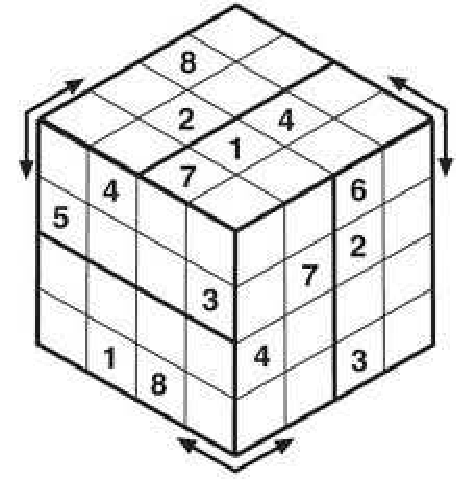
\includegraphics[width=0.3\textwidth]{images}
 \caption{这是一个图片测试例子(中)}
 \label{fig:amss1}
\end{figure}

该页是专门用来测试插入图片的方法,这个方法有很多种,需要自己花点时间来研究学习下,就像表格一样,
下面这只是一个简单的例子。好了,结束。

\subsection{图形位于页面上}
该页是专门用来测试插入图片的方法,这个方法有很多种,需要自己花点时间来研究学习下,就像表格一样,
下面这只是一个简单的例子。好了,结束。该页是专门用来测试插入图片的方法,这个方法有很多种,需要自己花点时间来研究学习下,就像表格一样,
下面这只是一个简单的例子。好了,结束。

\begin{figure}[t]
 \centering
 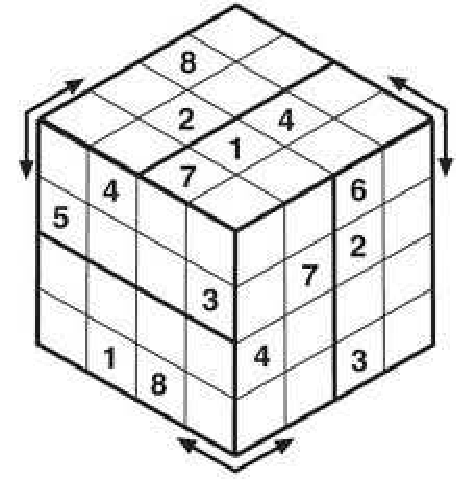
\includegraphics[width=0.3\textwidth]{images}
 \caption{这是一个图片测试例子(上)}
 \label{fig:amss2}
\end{figure}

该页是专门用来测试插入图片的方法,这个方法有很多种,需要自己花点时间来研究学习下,就像表格一样,
下面这只是一个简单的例子。该页是专门用来测试插入图片的方法,这个方法有很多种,需要自己花点时间
来研究学习下,就像表格一样,下面这只是一个简单的例子。该页是专门用来测试插入图片的方法,这个方法
有很多种,需要自己花点时间来研究学习下,就像表格一样,下面这只是一个简单的例子。

\subsection{图形位于页面下}
该页是专门用来测试插入图片的方法,这个方法有很多种,需要自己花点时间来研究学习下,就像表格一样,
下面这只是一个简单的例子。

\begin{figure}[b]
 \centering
 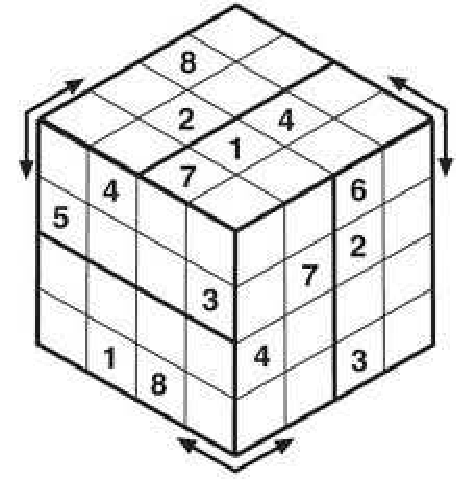
\includegraphics[width=0.3\textwidth]{images}
 \caption{这是一个图片测试例子(下)}
 \label{fig:amss3}
\end{figure}


该页是专门用来测试插入图片的方法,这个方法有很多种,需要自己花点时间来研究学习下,就像表格一样,
下面这只是一个简单的例子。该页是专门用来测试插入图片的方法,这个方法有很多种,需要自己花点时间
来研究学习下,就像表格一样,下面这只是一个简单的例子。

该页是专门用来测试插入图片的方法,这个方法
有很多种,需要自己花点时间来研究学习下,就像表格一样,下面这只是一个简单的例子。该页是专门用来测
试插入图片的方法,这个方法有很多种,需要自己花点时间来研究学习下,就像表格一样,
下面这只是一个简单的例子。

该页是专门用来测试插入图片的方法,这个方法有很多种,需要自己花点时间来研究学习下,就像表格一样,
下面这只是一个简单的例子。该页是专门用来测试插入图片的方法,这个方法有很多种,需要自己花点时间
来研究学习下,就像表格一样,下面这只是一个简单的例子。

该页是专门用来测试插入图片的方法,这个方法
有很多种,需要自己花点时间来研究学习下,就像表格一样,下面这只是一个简单的例子。该页是专门用来测
试插入图片的方法,这个方法有很多种,需要自己花点时间来研究学习下,就像表格一样,
下面这只是一个简单的例子。

该页是专门用来测试插入图片的方法,这个方法有很多种,需要自己花点时间来研究学习下,就像表格一样,
下面这只是一个简单的例子。该页是专门用来测试插入图片的方法,这个方法有很多种,需要自己花点时间
来研究学习下,就像表格一样,下面这只是一个简单的例子。该页是专门用来测试插入图片的方法,这个方法
有很多种,需要自己花点时间来研究学习下,就像表格一样,下面这只是一个简单的例子。该页是专门用来测
试插入图片的方法,这个方法有很多种,需要自己花点时间来研究学习下,就像表格一样,
下面这只是一个简单的例子。


    
\chapter{总结与展望}
\label{chap:con}

\subsection{总结}

\subsection{进一步工作}


    \appendix
    
\chapter[本科生毕业设计论文撰写规范]{西安电子科技大学本科生毕业设计论文撰写规范}
\label{chap:requires}
\section{毕业设计(论文)的总体要求}
撰写论文应简明扼要,一般不少于15000字(外语专业可适当减少,但不得少于10000单词,且须全部用外语书写)。

\section{毕业设计(论文)的编写格式}
每一章、节的格式和版面要求整齐划一、层次清楚。其中:
\begin{itemize}
  \item 论文用纸:统一用A4纸,与论文封皮,任务书,工作计划,成绩考核表一致。
  \item 章的标题:如:``摘要''、``目录''、``第一章''、``附录''等,黑体,三号,居中排列。
  \item 节的标题:如:``2.1  认证方案''、``9.5  小结''等,宋体,四号,居中排列。
  \item 正文:中文为宋体,英文为``Times News Roman'',小四号。正文中的图名和表名,宋体,五号。
  \item 页眉:宋体五号,居中排列。左面页眉为论文题目,右面页眉为章次和章标题。页眉底划线的宽度为0.75磅。
  \item 页码:宋体小五号,排在页眉行的最外侧,不加任何修饰。
\end{itemize}

\section{毕业设计(论文)的前置部分}
毕业设计(论文)的前置部分包括封面、中英文摘要、目录等。
\subsection{封面及打印格式}
\begin{itemize}
  \item 学号:按照学校的统一编号,在右上角正确打印自己的学号,宋体,小四号,加粗。
  \item 题目:题目应和任务书的题目一致,黑体,三号。
  \item 学院、专业、班级、学生姓名和导师姓名职称等内容,宋体,小三号,居中排列。
\end{itemize}

\subsection{中英文摘要及关键词}
摘要是关于论文的内容不加注释和评论的简短陈述,具有独立性和自含性。它主要是
简要说明研究工作的目的、方法、结果和结论,重点说明本论文的成果和新见解。关键词
是为了文献标引工作从论文中选取出来用以表示全文主题内容信息的术语。
\begin{enumerate}
  \item 中文摘要,宋体小四号,一般为300字;英文摘要,``Times News Roman''字
体,小四号,一般为300个实词。摘要中不宜出现公式、非公用的符号、术语等。
  \item 每篇论文选取3 \~{} 5个关键词,中文为黑体小四号,英文为``Times News Roman''字体加粗,小四号。关键词排列在摘要的左下方一行,起始格式为:``\textbf{关键词}:
      ''和``\textbf{Keyword:}''。具体的各个关键词以均匀间隔排列,之间不加任何分隔符号。
\end{enumerate}

\section{目录}
按照论文的章、节、附录等前后顺序,编写序号、名称和页码。目录页排在中英文摘要之后,主体部分必
须另页右面开始,全文以右页为单页页码。

\section{毕业设计(论文)的主体部分}
毕业设计(论文)的主体部分包括引言(绪论)、正文、结论、结束语、致谢、参考文献。
\subsection{绪论}
作为论文的开端,简要说明作者所做工作的目的、范围、国内外进展情况、前人研究成果、
本人的设想、研究方法等。
\subsection{正文} 为毕业设计(论文)的核心部分,包括理论分析、数据资料、实验方法、结果、本人的论点和结
论等内容,还要附有各种有关的图表、照片、公式等。要求理论正确、逻辑清楚、层次分明、文字流畅、数据真实可
靠,公式推导和计算结果无误,图表绘制要少而精。
\begin{description}
  \item[图] 包括曲线图、示意图、流程图、框图等。图序号一律用阿拉伯数字分章依序编码,如:图1.3、图2.11。每一图应有简短确切的
      图名,连同图序号置于图的正下方。图中坐标上标注的符号和缩略词必须与正文中一致。
  \item[表] 包括分类项目和数据,一般要求分类项目由左至右横排,数据从上到下竖列。分类项目横排中必须标明符号或单位,竖列的数据栏中不宜出现``同上'' 、``同左''等类似词语,一律填写具体的数字或文字。表序号一律用阿拉伯数字分章依序编码,如:表2.5、表10.3。每一表应有简短确切的题名,
      连同表序号置于表的正上方。
  \item[公式] 正文中的公式、算式、方程式等必须编排序号,序号一律用阿拉伯数字分章依序编码,如:式(3-32)、式(6-21)。对于较长的公式,另行居中横排,只可在符号处(如:+、-、*、/、$<$、 $>$等)转行。公式序号标注于该式所在行(当有续行时,应标注于最后 一行)的最右边。连续性的公式在``=''处排列整齐。大于999的整数或多于三位的小数,一律用半个阿拉伯数字符的小间隔分开;小于1的数应将0置于小数点之前。
  \item[计量单位] 单位名称和符号的书写方式一律采用国际通用符号。
\end{description}

\subsection{结论}
是对主体的最终结论,应准确、完整、精炼。阐述作者创造性工作在本研究领域的地位和作用,对存在的问题和不足应给予客观的说明,也可提出进一步的设想。

\subsection{致谢}
对协助完成论文研究工作的单位和个人表示感谢。

\subsection{参考文献}
在学位论文中引用参考文献时,引出处右上角用方括号标注阿拉伯数字编排的序号(必须与参考文献一致)。参考文献的排列格
式分为:
\begin{description}
  \item[专著类的文献] [序号]  作者 . 专著名称.  版本. 出版地:出版者,出版年. 参考的页码。
  \item[期刊类的文献] 作者 . 文献名. 期刊名称.  年 , 月,  卷(期). 页码。
\end{description}
其中作者采用姓在前、名在后的形式。当作者超过三个时,只著录前三个人,其后
加``等''字即可。

\section{毕业设计(论文)的附录部分}
附录是作为学位论文主体的补充,包括下列内容:
\begin{enumerate}
  \item 正文中过于冗长的公式推导;
  \item 为读者阅读方便所需要的辅助性的数学工作或带有重复性的图表;
  \item 由于过分冗长而不宜在正文中出现的计算机程序清单;
  \item 对于一般读者并非必要阅读,但对本专业同行有参考价值的资料。
  \item 附录编于正文后,与正文连续编页码,每一附录均另页起。
  \item 附录依次用大写正体A,B,C……编序号,黑体,三号。如:附录A。
  \item 附录中的图、表、式、参考文献等与正文分开,用阿拉伯数字另行编序号,注意在数码前冠以附录的
      序码。如:图A1;表B2;式(C-3);文献[D5]。
\end{enumerate}
\section{毕业设计(论文)的打印规格}
论文正文页面和版面的设置规格:论文正文双面打印,为了便于装订、复制,要求每页纸的四周留有足够的空白边缘。以WORD97为例:

页面设置数据为:上3厘米、下2厘米、内侧3厘米、外侧2厘米;装订线 -- 1厘米;页眉  - 2厘米;  页脚 - 1厘米。

版面设置数据为:文字的行间距 - 1. 5倍 ;  公式的行间距 - 1. 5倍字符间距 - 标准;页码数据-对称页边距。

\section{毕业设计(论文)的装订说明}
毕业设计(论文)要求以A4纸的标准,按照下列顺序装订。外文资料翻译原文及译文另册装订,格式参照论文对应内容格式要求。

\begin{enumerate}
  \item 封面
  \item 任务书
  \item 工作计划
  \item 中期检查表
  \item 成绩考核登记表
  \item 中、外论文摘要
  \item 目录
  \item 引言
  \item 论文
  \item 结论
  \item 结束语
  \item 参考文献
  \item 附录
\end{enumerate}












%%----------------- 附件部分 ----------------- %%
    \backmatter
    \ifx\allfiles\undefined
\documentclass{XDBAthesis}
\def\pictures{}
\begin{document}
\else
\fi

\begin{thanks}

毕业论文暂告收尾,这也意味着我在西安电子科技大学的四年的学习生活既将结束。回首既往,自己一生最宝贵的时光能于这样的校园之中,能在众多学富五车、才华横溢的老师们的熏陶下度过,实是荣幸之极。在这四年的时间里,我在学习上和思想上都受益非浅。这除了自身努力外,与各位老师、同学和朋友的关心、支持和鼓励是分不开的。

首先感谢霍红卫教授的指导,霍老师在我论文写作期间给了我莫大的帮助。从选题到构思,研究,撰写,每一步都倾注了霍老师大量的心血。

其次感谢陈晓阳学长,每次在我迷茫时都给我指明了方向。特别是研究遇到一些瓶颈时,陈学长都会用其丰富的经验帮我度过。

感谢ShaSha教授,提供了GraphGrep源代码。

时间的仓促及自身专业水平的不足,整篇论文肯定存在尚未发现的缺点和错误。
恳请阅读此篇论文的老师、同学,多予指正,不胜感激!


\end{thanks}

\ifx\allfiles\undefined
%\bibliographystyle{unsrt}
\bibliography{main}
\end{document}
\fi
    
\fontsize{10.5pt}{10.5pt}\selectfont
\begin{thebibliography}{10}

\bibitem{site:ctex}
 http://www.ctex.org


\bibitem{lshort-cn}
\CTeX{}~翻译小组.
\newblock {lshort~中文版~}.
\newblock (2003)


\bibitem{deng:01a}
{邓建松,~彭冉冉,~陈长松}.
\newblock {\LaTeXe{}~科技排版指南}.
\newblock 科学出版社,~书号:~7-03-009239-2/TP.1516, 北京, (2001).

\bibitem{wang:00a}
王磊.
\newblock {\LaTeXe{}~插图指南}.
\newblock (2000).

\bibitem{zhang:03a}
张林波.
\newblock {于新版~CCT~的说明}.
\newblock (2003).

\bibitem{knuth86e}
Donald~E, Knuth.
\newblock {Computer Modern Typefaces}, volume~E of {Computers and
  Typesetting}.
\newblock Addison-Wesley, Reading, Massachusetts, (1986).

\bibitem{knuth86d}
Donald~E. Knuth.
\newblock {{METAFONT}: The Program}, volume~D of {Computers and
  Typesetting}.
\newblock Addison-Wesley, Reading, Massachusetts, (1986).

\bibitem{knuth86c}
Donald~E. Knuth.
\newblock {The {METAFONT}book}, volume~C of {Computers and
  Typesetting}.
\newblock Addison-Wesley, Reading, Massachusetts, (1986).

\bibitem{knuth86b}
Donald~E. Knuth.
\newblock {{\TeX}: The Program}, volume~B of { Computers and
  Typesetting}.
\newblock Addison-Wesley, Reading, Massachusetts, (1986).

\bibitem{knuth86a}
Donald~E. Knuth.
\newblock {The {TeX}book}, volume~A of {Computers and Typesetting}.
\newblock Addison-Wesley, Reading, Massachusetts, (1986).

\bibitem{lamport85a}
Leslie Lamport.
\newblock {{\LaTeX} --- A Document Preparation System: User's Guide and
  Reference Manual}.
\newblock Addison-Wesley, Reading, Massachusetts, 2nd edition, (1985).

\end{thebibliography}


\end{document}



